\documentclass[11pt]{article}

\usepackage{amsmath, amssymb, amsthm}
\usepackage{tikz}

\theoremstyle{plain}
\newtheorem{thm}{Theorem}[section]
\newtheorem*{thm*}{Theorem}
\newtheorem{prop}[thm]{Proposition}
\newtheorem{lem}[thm]{Lemma}
\newtheorem*{lem*}{Lemma}
\newtheorem{dfn}[thm]{Definition}
\newtheorem{cor}[thm]{Corollary}
\newtheorem{claim}[thm]{Claim}
\newtheorem{conj}[thm]{Conjecture}
\newtheorem{ques}[thm]{Question}
\newtheorem*{rem}{Remark}


\oddsidemargin  0pt
\evensidemargin 0pt
\marginparwidth 40pt
\marginparsep 10pt
\topmargin 0pt
\headsep 10pt
\textheight 8.2in
\textwidth 6.4in
\renewcommand{\baselinestretch}{1.1}

\newcommand{\codeg}{\text{codeg}}
\newcommand{\BBE}{\mathbb{E}}
\newcommand{\BFP}{\mathbf{P}}
\usepackage{amsmath}
\usepackage{amsthm}
\usepackage{amssymb}
\usepackage{mathtools}
\usepackage{hyperref}
\usepackage{url}





\usepackage{graphicx}
\usepackage{caption}
\usepackage{subcaption}

\def\eQb#1\eQe{\begin{eqnarray*}#1\end{eqnarray*}}
\def\eQnb#1\eQne{\begin{eqnarray}#1\end{eqnarray}}
\providecommand{\e}[1]{\ensuremath{\times 10^{#1}}}
\providecommand{\pb}[0]{\pagebreak}
\DeclarePairedDelimiter\ceil{\lceil}{\rceil}
\DeclarePairedDelimiter\floor{\lfloor}{\rfloor}

\newcommand{\E}{\mathrm{E}}
\newcommand{\Var}{\mathrm{Var}}
\newcommand{\Cov}{\mathrm{Cov}}

\def\Qb#1\Qe{\begin{question}#1\end{question}}
\def\Sb#1\Se{\begin{solution}#1\end{solution}}


\newtheoremstyle{quest}{\topsep}{\topsep}{}{}{\bfseries}{}{ }{\thmname{#1}\thmnote{ #3}.}
\theoremstyle{quest}
\newtheorem*{definition}{Definition}
\newtheorem*{theorem}{Theorem}
\newtheorem*{lemma}{Lemma}
\newtheorem*{question}{Question}
\newtheorem*{preposition}{Preposition}
\newtheorem*{exercise}{Exercise}
\newtheorem*{challengeproblem}{Challenge Problem}
\newtheorem*{solution}{Solution}
\newtheorem*{remark}{Remark}
\usepackage{verbatimbox}
\usepackage{listings}
\usepackage{mathrsfs}
\date{}
\title{\vspace{-0.7cm}
PDE II: Final}

\author{
Youngduck Choi 
\thanks{Department of Mathematics, Courant Institute of Mathematical Sciences, 
yc1104@nyu.edu; If you find an error and want to share with me, 
you can reach me via email.
}}

\begin{document}

\maketitle

\begin{abstract}
This work contains solutions for the final of the PDE II course at Courant.
\end{abstract}


\begin{question}[1-1]
\hfill
\begin{figure}[h!]
  \centering
    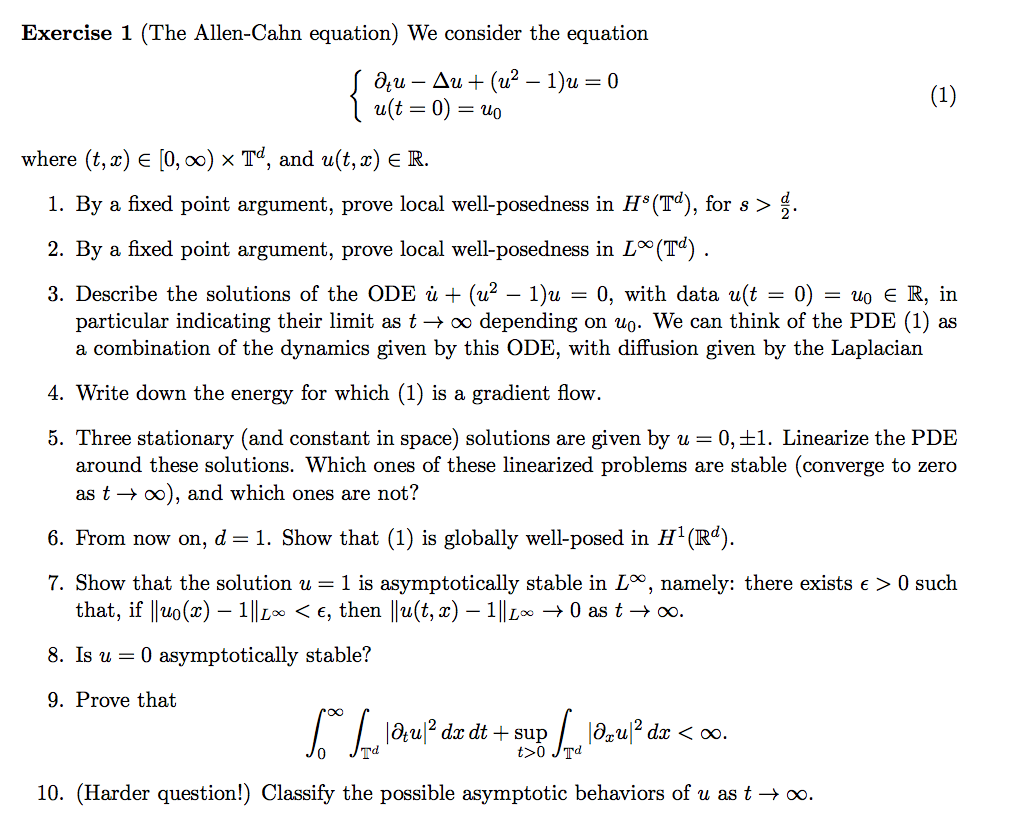
\includegraphics[width=0.7\textwidth]{pde2-f-p1.png}
\end{figure}
\end{question}
\begin{solution} \hfill \\
\textbf{(1)} We will roughly 
follow the strategy shown in class with the cubic NLH problem.
By definition, our solution of the equation will be
functions in $C([0,T],H^s)$ such that 
\eQb
u(t) &=& e^{t\triangle} u_0 + \int_{0}^{t}e^{(t-s)\triangle} (u - u^3) ds 
\eQe
for some $T > 0$. This in turn can be rewritten as a fixed point problem:
\eQnb
u &=& Ru \>\>\> \text{with} \>\>\> R:C([0,T],H^s) \to C([0,T],H^s), \>\>\> 
v \mapsto u \nonumber \\ 
&\text{and}&  \>\>\> 
u = e^{t\triangle} u_0 + \int_{0}^{t} e^{(t-l)\triangle} (v(l) - v(l)^3) dl.
\label{eq:1-1-1} 
\eQne
for some $T > 0$.
Set $\rho = ||u_0||_{H^s}$. We claim that there exists $T,K$ suitably chosen
such that $R$ is a contraction in $B_{(C[0,T],H^s)}(0,K\rho)$. We compute, for
any $u \in B_{(C[0,T],H^s)}(0,K\rho)$, 
\eQnb
||R(u)||_{C([0,T],H^s)} &\leq& ||u_0||_{H^s} + \sup_{0 < t < T} \int_{0}^{t} 
||e^{(t-l)\triangle}(u - u^3)(l)||_{H^s} dl  \nonumber \\
&\leq& \rho + CT \sup_{0 < t < T} (||u||_{H^s} + ||u||_{H^s}^3) \label{eq:1-1-2} \\
&\leq& \rho + CT (K\rho + K^3 \rho^3) \label{eq:1-1-3}  
\eQne 
where $C$ is an universal constant independent of $u$, whose existence is 
justified along with~\eqref{eq:1-1-2}  
from the fact that $e^{t\triangle}$ is bounded
on $H^s$ for each $t > 0$ and $H^s$ is an algebra for each $s > \dfrac{d}{2}$, 
and~\eqref{eq:1-1-3} follows
from $u \in B_{C([0,T],H^s)}(0, K\rho)$. Hence, if 
\eQb
CT(K\rho + K^3\rho^3) < (K-1)\rho &\iff& T \leq \dfrac{K-1}{C(K + K^3\rho^2)} 
\eQe 
then, $R$ stabilizes $B_{C([0,T],H^s)}(0,K\rho)$. We now investigate
the condition on $K$ and $T$, which will imply that $R$ is a contraction in
$B_{C([0,T],H^s)}(0,K\rho)$ 
i.e. for any $u, v \in B_{C([0,T],H^s)}(0,K\rho)$, 
\eQb
||Ru - Rv||_{C([0,T],H^s)} < \dfrac{1}{2} ||u - v||_{C([0,T],H^s)}.
\eQe
We compute, for any $u,v \in B_{C[0,T],H^s)}(0,K\rho)$, with the same reasoning as above,
\eQb
\sup_{0 < t < T} ||R(u)(t) - R(v)(t)||_{H^s} &\leq& 
\sup_{0 < t < T} \int_{0}^{t} ||e^{(t-l)\triangle}(u(l) - u^3(l) - v(l) + v^3(l)) ||
dl  \\
&=& 
\sup_{0 < t < T} \int_{0}^{t} ||e^{(t-l)\triangle}(v(l)- u(l))(v^2(l) + v(l)u(l)
+ u^2(l) - 1)|| dl \\
&\leq& C \sup_{0 < t < T} \int_{0}^{t} ||u(l)-v(l)||( (||u(l)|| + ||v(l)||)^2 + 1) dl \\
&\leq& C (K^2\rho^2 + 1) T ||u - v||_{C([0,T],H^s)}.  
\eQe
Hence, 
\eQb
T \leq \dfrac{1}{2C(K^2\rho^2 +1)} &\implies& \>\>\> R \>\>\> \text{is a contraction on} 
\>\>\>  B_{C([0,T],H^s)}(0, K\rho).
\eQe
Therefore, choose any $K > 1$, and then choose
\eQb
T &=& \min\{\dfrac{K-1}{C(K + K^3\rho^2}, \dfrac{1}{2C(K^2\rho^2 + 1)}\}. 
\eQe
Now, with respect to these choices, by a general fixed point theorem, we have
proved existence and uniqueness in $B_{C([0,T],H^s}(0,K\rho)$. Continuous dependence
on the data and uniqueness on the whole space $C([0,T],H^s)$ can be argued in the same
way as the lecture note 7. So we are done. \hfill $\qed$

\bigskip

\noindent \textbf{(2)}
As $L^{\infty}$ is an algebra, the technique used above will work if we show that
for each $t > 0$
\eQb
 e^{t\triangle} \>\>\> \text{is bounded on} \>\>\> L^{\infty}. 
\eQe

\bigskip 

\noindent \textbf{(3)} We solve the given ODE. Observe that
\eQb
\dfrac{1}{u - u^3} = \dfrac{1}{u} + \dfrac{u}{1 - u^2}.
\eQe 
Hence, 
\eQb
du = 
\eQe
so
\eQb
u(t) = \ln|t| - \dfrac{1}{2} \ln| (1-t)(1+t) | + u_0  
\eQe

\bigskip

\noindent \textbf{(4)} We derive the energy formally, as shown in class. Multiplying
by $u_t$ on both sides of the equation, and integrating by parts,
\eQb
\int u_t \partial_t u - u_t \triangle u + u_t u^3 - u_t u  = 0 
\eQe
so
\eQb
\int |\partial_t u |^2 dx &=& - \dfrac{d}{dt}
(\dfrac{1}{4} \int u^4  dx 
- \dfrac{1}{2} \int u^2 dx + \dfrac{1}{2} |\triangle u|^2 dx). \\
\eQe
Therefore,
\eQb
E(u) &=&
\dfrac{1}{4} \int u^4  dx 
- \dfrac{1}{2} \int u^2 dx + \dfrac{1}{2} |\triangle u|^2 dx, \\
\eQe
as required. \hfill $\qed$

\bigskip

\noindent \textbf{(5)}
Let $u = 0$. Ignoring the non-linear term in $u - u^3$, we get the linearized pde as
\eQb
\partial_t - \triangle u = u.
\eQe
Let $u = 1$. Set $v = u - 1$, so  
\eQb
\partial_t v - \triangle v &=& \partial_t u - \triangle u = (v+1)^2 - (v+1)^3 \\
&=& -v^3 - 3v^2 - 2v.
\eQe
Ignoring the nonlinear term, we get the linearized pde as 
\eQb
\partial_t v - \triangle v = -2v. 
\eQe
Similarly, for $u = -1$, we get the linearized pde as
\eQb
\partial_t v - \triangle v = -2v. 
\eQe
For the $u = 0$ case, set $u = e^{t} v$ to get
\eQb
u(x,t) &=& e^{t} \int \Phi(x-y,t) u_0(y) dy
\eQe
where $\Phi$ is the heat kernel. Then, for any $\delta > 0$, and $||u_0||_{H^s} < \delta$
such that $u \neq 0$, $u(x,t)$ blows up by the fact that $e^t$ term dominates.
For the other two cases, we have $e^{-2t}$ factor instead of $e^t$, so we see that
the linearized PDE is unstable for $u = 0$ and stable for $u = \pm 1$. \hfill
$\qed$

\bigskip

\noindent 
\textbf{(6)} As $ s = 1 > \dfrac{1}{2} = \dfrac{d}{2}$, by 1, we have local 
well-posedness of the equation in $H^1(\mathbb{T})$. Let $T^*$ be the maximal 
time of existence $T^*$. Now, observe that by Soblev embedding, we have 
\eQb
u_0 \in H^{1}(\mathbb{T}) \subset 
C^{\frac{1}{2}}(\mathbb{T}) \subset C(\mathbb{T}) \subset L^{\infty}(\mathbb{T})
\subset \bigcap_{1 \leq p} L^{p}(\mathbb{T}).
\eQe 
Therefore, $E(u_0) < \infty$, and since the energy is decreasing 
\eQb
\sup_{0 < t < T^*} ||u(t)||_{H^1} &\leq& C \sup_{0 < t < T^*} (||u(t)||_{L^2} 
+ ||\triangledown u(t)||_{L^2} )) \\
&\leq& \\
&\leq& C \sup_{0 < t < T^*} E(u(t)) \leq C E(u_0) \leq 
\eQe

Hence $u$ is globally bounded in $H^1$, so
\eQb
\limsup_{t \to T^*} ||u(t)||_{H^1} < \infty
\eQe
and by the lemma in page 2 of lecture note 8, $T^* = \infty$.

\end{solution}

\newpage

\begin{question}[1-2]
\hfill
\begin{figure}[h!]
  \centering
    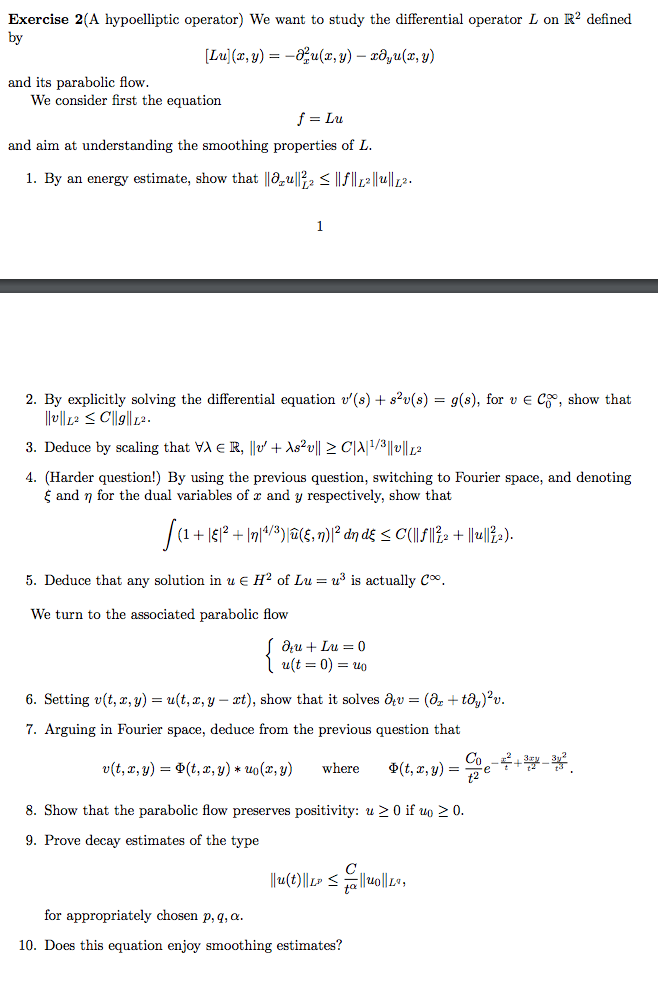
\includegraphics[width=0.7\textwidth]{pde2-f-p2.png}
\end{figure}
\end{question}
\begin{solution} \hfill \\

\newpage

\noindent \textbf{(1)} We proceed by our usual formal derivation of the energy estimate.
Multiplying both sides of the equation
by $u$, integrating over $x,y$, and integrating by parts,
\eQb
\int \int uf dx dy &=& -\int\int uu_{xx} dx dy - \int \int u x u_y dy dx \\
&=& \int\int (u_x)^2 dx dy - \int x (\dfrac{1}{2} u^2|_{-\infty}^{\infty}) dx \\
&=& \int\int (u_x)^2 dx dy 
\eQe
and hence, by Holder's inequality,
\eQb
||u_x||_{L^2}^2 = |\int \int uf dx dy | \leq \int\int |uf| dx dy \leq ||f||_{L^2}
||u||_{L^2}, 
\eQe
as required. \hfill $\qed$

\bigskip

\noindent \textbf{(2)}
Firstly, observe that as $v$ vanishes at $\infty$, if $g$ solves the ODE then,
$g$ has compact support. Now, we solve the ODE. Multiplying both sides of the
equation by $e^{\frac{1}{3} s^3}$(integrating factor),
\eQb
e^{\frac{1}{3}s^3} dv + e^{\frac{1}{3}s^3} s^2 v ds &=& e^{\frac{1}{3} s^3} g(s) ds
\eQe 
and hence
\eQb
e^{\frac{1}{3} s^3} g(s) ds = d(e^{\frac{1}{3}s^3}v).
\eQe
Therefore,
\eQb
v(s) = e^{-\frac{1}{3} s^3} \int_{0}^{s} g(t) e^{\frac{1}{3} t^3} dt .
\eQe
solves the ODE. Now, we compute 
\eQb
||v||_{L^2}^2 &=& 
\int (e^{-\frac{1}{3} s^3} \int_{0}^{s} g(t) e^{\frac{1}{3} t^3} 
dt)^2 ds 
\leq
\int (e^{-\frac{1}{3} s^3} \int_{0}^{s} g(t) e^{\frac{1}{3} s^3} 
dt)^2 ds \\
&=& \int  (\int_{0}^{s} g(t) dt)^2 ds  
\leq \int  (\int_{\mathbb{R}} |g(t)| dt)^2 ds  \\  
&\leq& \int \int_{\mathbb{R}} |g(t)|^2 dt ds 
\leq m(\text{supp}(v)) ||g||_{L^2}^2 \\ 
\eQe
where the second last inequality holds by Jensen's inequality on finite measure space,
as $g$ has compact support, and $m(\text{supp}(v)) < \infty$ by assumption. \hfill 
$\qed$

\bigskip \noindent \textbf{(3)}  


\bigskip
\noindent \textbf{(4)} 
From the energy estimate (1), and taking the Fourier transform of $\partial_x u$,
\eQb
\int\int |\xi|^2 |\hat{u}(\xi,\eta)|^2 d\xi d\eta &=& ||\partial_x||_{L^2}^2 
\leq ||\hat{f}||_{L^2} ||\hat{u}||_{L^2} \leq \dfrac{1}{2}(||\hat{f}||_{L^2}^2 +
||\hat{u}||_{L^2}^2)  
\eQe
and hence, for some constant $C$,
\eQb
\int\int (1+|\xi|^2) |\hat{u}|^2 &\leq& C(||\hat{f}||_{L^2} + ||\hat{u}||_{L^2}).
\eQe
Therefore, it suffices to show that, for some constant $C > 0$, 
\eQnb
\int\int |\eta|^{\frac{4}{3}} |\hat{u}(\xi, \eta)|^2 d\xi d\eta &\leq& 
C ||\hat{f}||_{L^2}^2 \label{eq:1-2-4-1}  
\eQne
Taking the Fourier transform of the equation,
\eQb
|\xi|^2 \hat{u} + \eta \partial_{\xi} \hat{u} = \hat{f}
\eQe
and dividing both sides of the above equation by $\eta$,
\eQb
\dfrac{1}{\eta} |\xi|^2 \hat{u} +  \partial_{\xi} \hat{u} = \dfrac{1}{\eta} \hat{f}.
\eQe
Now, by the scaling estimate from $(3)$, for some constant $C_1 > 0$,
\eQb
|\dfrac{1}{\eta}| ||\hat{f}(\xi,\eta)||_{L^2_{\xi}} &\geq& C_1 |\eta|^{-\frac{1}{3}} 
||\hat{u}(\xi,\eta)||_{L^2_{\xi}}
\eQe
and hence, rearranging and squaring both sides, for some constant $C_2 > 0$.
\eQb
C_2 \int |\hat{f}(\xi, \eta)|^2 d\xi &\geq&  
|\eta|^{\frac{4}{3}} \int |\hat{u}(\xi,\eta)|^2 d\xi. 
\eQe
Integrating the above equation with respect to $\eta$ gives~\eqref{eq:1-2-4-1},
so we are done. \hfill $\qed$

\bigskip
\noindent \textbf{(5)} 


\bigskip
\noindent \textbf{(6)} We wish to show that
\eQnb
v_t &=& v_{xx} + 2tv_{xy} + t^2 v_{yy} \label{eq:1-2-6-1} 
\eQne
To that end, we compute
\eQb
v_x &=& u_x - tu_y \\
v_{xx} &=& u_{xx} - 2tu_{yx} + t^2 u_{yy} \\
v_t &=& u_t - xu_y \\
2tv_{xy} &=& 2tu_{xy} - 2t^2 u_{yy} \\
t^2 v_{yy} &=& t^2 u_{yy}.
\eQe
Substituting the above equations to~\eqref{eq:1-2-6-1},
\eQb
u_t - xu_y &=& u_{xx} = u_{xx} - 2tu_{xy} + t^2 u_{yy} + 2tu_{xy} - 2t^2 u_{yy}
+ t^2 u_{yy}
\eQe
which simplifies to
\eQb
u_t - u_xx - xu_y &=& 0.
\eQe
Therefore, we see that $v$ solves~\eqref{eq:1-2-6-1}, as required. \hfill $\qed$


\bigskip 

\noindent \textbf{(8)} Suppose $u_0 \geq 0$. Note that $\Phi$ is non-negative
everywhere. Hence, by 6 and 7, for each $t,x,y$,  
\eQb
u(t,x,y) &=& v(t,x,y+xt)  = \Phi(t,x,y+xt)* u_0(x,y+xt) \geq 0,
\eQe
as required. \hfill $\qed$


\end{solution}

\end{document}

